\documentclass[11pt,a4paper]{scrartcl}
\typearea{12}
\usepackage{graphicx}
\usepackage{pstricks}
\usepackage{listings}
\lstset{language=python}
\pagestyle{headings}
\markright{Computation Neuroscience - 7 vision}

\usepackage{tikz}
\usepackage{tikzscale}
\usepackage{pgfplots}
\usepackage{color}
\usepackage{pgf}
\usepackage[utf8]{inputenc}
\usetikzlibrary{arrows,automata}
\usetikzlibrary{positioning}


\begin{document}

\section*{Vision}

\subsection*{Introduction} 
This lecture is about vision, when they are complete they will discuss
how simple cells in V1 are modelled and how their behavior may be
explained by sparseness, at the moment they only contain the
introduction.

\subsection*{The visual pathway}
The visual system starts at the eye, where photons are detected and
some denoising occurs; the optical nerve then carries the information
to the thalamus, in the very center of the brain, there it is further
processed and denoised before being relayed on to the visual cortex,
at the very back of the cortex. As it is processed in stages in the
cortex the information is passed forward through the cortex, as
objects are recognized the information fans out and is integrated with
other signals, from memory, from other sensory modalities and other
aspect of our cognition. The basic pathway is shown in an very old
drawing in Fig.~\ref{fig:Fabrica} and is summarized in
Fig.~\ref{fig:pathway}. One notable aspect is that different sides
of the brain deal with different sides of the visual field, so signal
from the left sides of the retina of both eyes go to the right side of
the brain and signals from the right sides so to the left side.

\begin{figure}
\begin{center}
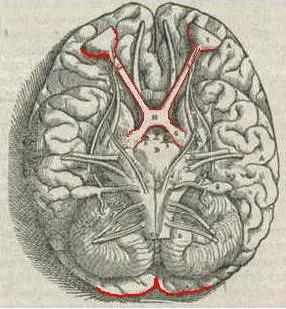
\includegraphics[width=7cm]{Fabrica_VisualSystem.jpg}
\end{center}
\caption{The visual pathway. This is an old drawing due to the C16
  Belgian anatomist Andreas Vesalius taken from his influential 1543
  textbook \textsl{De Humani Corporis Fabrica}. In red are marked the
  retina, the optic nerves, the thalamus where they cross and the
  primary visual cortex. [Image from Wikipedia].\label{fig:Fabrica}}
\end{figure}


Light is detected at the retina, the retina is a surprising organ in
that it is backwards compared to how you'd expect it to be organized;
the layer with light detectors is at the back instead of the
front. Leaving that aside though, basically light is detected in
specialized cells called \textsl{photoreceptors}, these don't spike,
but they do convert light into electrical activity; this is passed
forward though \textsl{bipolar cells} to \textsl{ganglion
  cells}. Ganglion cells aggregate activity from a number of
photoreptors, along with activity from some inhibitory cells in the
intermediate layer and their axons form the optic nerve, carrying
information to the thalamus. A sketch of the retina is given in Fig.~\ref{fig:retina}.

\begin{figure}
\begin{center}
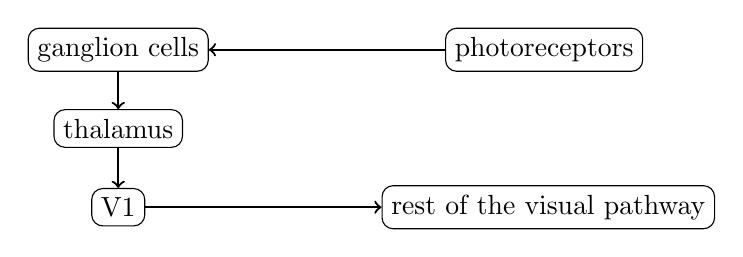
\begin{tikzpicture}
\node[rectangle,rounded corners,draw=black](ph){photoreceptors};
\node[rectangle,rounded corners,draw=black,left = 3cm of ph](g){ganglion cells};
\node[rectangle,rounded corners,draw=black,below of= g](th){thalamus};
\node[rectangle,rounded corners,draw=black,below of= th](v1){V1};
\node[rectangle,rounded corners,draw=black,right = 3cm of v1](v){rest of the visual pathway};
\path (ph) edge[->,thick] (g);
\path (g) edge[->,thick] (th);
\path (th) edge[->,thick] (v1);
\path (v1) edge[->,thick] (v);
\end{tikzpicture}
\end{center}
\caption{The visual pathway. This is a very rough diagram showing the visual pathway; V1 is the first visual area in the cortex.\label{fig:pathway}}
\end{figure}

\begin{figure}
 \begin{center}
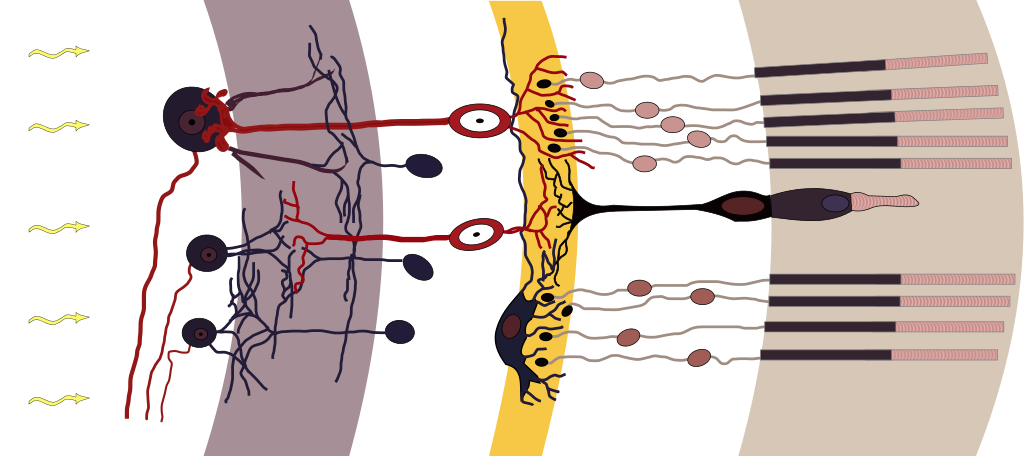
\includegraphics[width=12cm]{retina.png}
\end{center}
\caption{Rods, cones and nerve layers in the retina. The front of the eye is on the left. Light (from the left) passes through several transparent nerve layers to reach the rods and cones (far right). A chemical change in the rods and cones send a signal back to the nerves. The signal goes first to the bipolar and horizontal cells (yellow layer), then to the amacrine cells and ganglion cells (purple layer), then to the optic nerve fibres. The signals are processed in these layers. First, the signals start as raw outputs of points in the rod and cone cells. Then the nerve layers identify simple shapes, such as bright points surrounded by dark points, edges, and movement. (Based on a drawing by Ramón y Cajal, 1911.) [Caption and drawing taken from Wikipedia: Cajal derivative work: Anka Friedrich via Wikimedia Commons]\label{fig:retina}}
\end{figure}

\subsection*{Receptive fields}
\textsl{Receptive fields} are often described as the stimuli giving
the largest response from a neuron. For ganglion and thalamic cells
these are contrast patches, see Fig.~\ref{fig:rf_ganglion}, in
\textsl{on-cells} small patches of the visual field where an
illuminated region surrounded by an unilluminated one causes firing,
different cells will respond to different locations. The width of the
receptive fields vary from the size of full stop at reading distance
in the center, to the size of a page near the periphery. In
\textsl{off-cells} the contrast is reverse, the cell responds to an
unilluminated region surrounded by an illuminated region. In V1 there
are cells called \textsl{simple cells} and cells called
\textsl{complex cells}; we will concentrate on the simple cells, these
have edge-like receptive fields; different cells respond to particular
orientations in particular locations in the visual field. 

The edge-like receptive fields in V1 were first discovered by Hubel
and Wiesel \cite{HubelWiesel1962a}. The used an electrode to record
from V1 neurons in anaesthetised cat; the moved an edge-like stimulus
around until they found the position that caused the highest firing
rate, they observed that the firing rate depended on orientation as
well as position, see Fig.~\ref{fig:hw} and Fig.~\ref{fig:hw_rf}.

\begin{figure}
\begin{center}

\begin{tikzpicture}
\node[rectangle,text width=3cm,text height=3cm,fill=gray](out1){};
\node[circle,text width=2cm,fill=black](surr1){};
\node[circle,text width=1cm,fill=white](cent1){};
\node[rectangle,text width=3cm,text height=3cm,fill=gray,right = 1cm of out1](out2){};
\node[circle,text width=2cm,fill=white,right = 2cm of surr1](surr2){};
\node[circle,text width=1cm,fill=black,right = 3cm of cent1](cent2){};
\end{tikzpicture}
\end{center}
\caption{On and off cells respond to small contrast patches. \label{fig:rf_ganglion}}
\end{figure}

\begin{figure}
\begin{center}

\begin{tikzpicture}
\node[rectangle,text width=3cm,text height=3cm,fill=gray](out1){};
\draw(0.25,0)[rotate=35,fill=black,draw=gray] ellipse (0.25cm and 0.85cm);
\draw(-0.25,0)[rotate=35,fill=white,draw=gray] ellipse (0.25cm and 0.85cm);

\node[rectangle,text width=3cm,text height=3cm,fill=gray,right = 1cm of out1](out2){};
\draw(4.75,0)[rotate around = {35:(4.25,0)},fill=white,draw=gray] ellipse (0.25cm and 0.85cm);
\draw(3.75,0)[rotate around = {35:(4.25,0)},fill=white,draw=gray] ellipse (0.25cm and 0.85cm);
\draw(4.25,0)[rotate around = {35:(4.25,0)},fill=black,draw=gray] ellipse (0.25cm and 0.85cm);
\end{tikzpicture}
\end{center}
\caption{Simple cells in V1 respond to edges.\label{fig:rf_v1}}
\end{figure}

\begin{figure}
\begin{center}
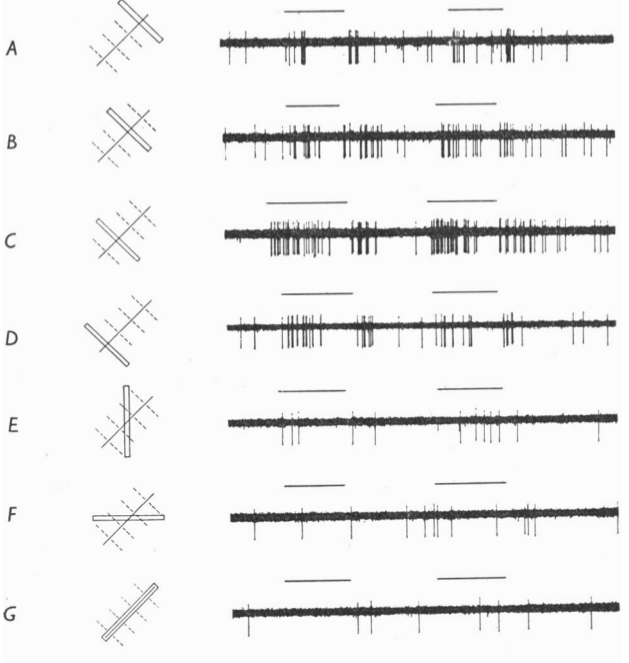
\includegraphics[width=12cm]{HW.png}
\end{center}
\caption{Experimental results from Hubel and Wiesel; the stimulus is a slit that allows light through from a souce, it is $0.125^\circ\times 2.5^\circ$ and is presented during the one-second period marked by the two bars over the plots. In the plots the vertical lines correspond to spikes. [Image from \cite{HubelWiesel1962a}].\label{fig:hw}}
\end{figure}


\begin{figure}
\begin{center}
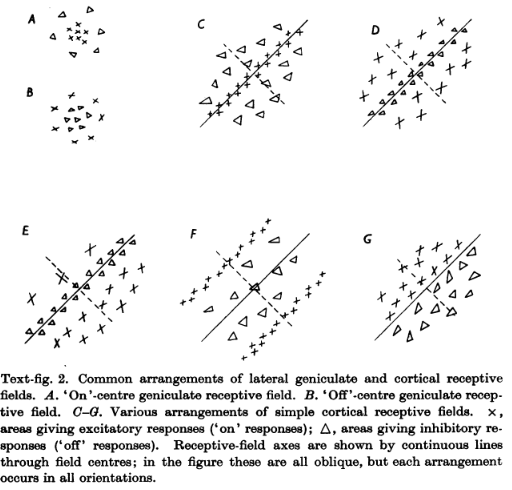
\includegraphics[width=12cm]{HW_rf.png}
\end{center}
\caption{More experimental results from Hubel and Wiesel; here they have mapped out the excitatory (crosses) and inhibitory (triangles) areas for a number of neurons. [Image from \cite{HubelWiesel1962a}].\label{fig:hw_rf}}
\end{figure}


\subsection*{Linear models}


One way to think about it is to imagine the entries in the receptive
field are synapse strengths for inputs from cells responding to
illumination at points in the visual field. To formalize this consider
linear models of the neuron's activity. Let $I_{ij}$ denote the
illumination level at point $(i,j)$ in the visual field, $i$ and $j$
are discrete coordinates, for simplicity we will treat everything
discretely. Now, imagine a linear model of the activity of the neuron,
with the firing rate depending linearly on the illuminations; leaving
out any messing with the firing rate having to be positive, this means
\begin{equation}
\tilde{r}=r_0+\sum w_{ij}I_{ij}
\end{equation}
where $r_0$ is the background firing rate and $w_{ij}$ give the
receptive field. Of course the firing rate of a neuron doesn't satisfy
a linear model but the idea is to choose the linear model which best
approximates the neuron, that is, for example, to choose $w_{ij}$ to
minimize the average square error $\langle (r-\tilde{r})^2\rangle$
between $r$, the observed firing rate and $\tilde{r}$ is the estimated
firing rate from the linear model.

As an example consider
\begin{equation}
[w_{ij}]=\left(\begin{array}{ccccc}
0&0&0&0&0\cr
0&-1/8&-1/8&-1/8&0\cr
0&-1/8&1&-1/8&0\cr
0&-1/8&-1/8&-1/8&0\cr
0&0&0&0&0\end{array}
\right)
\end{equation}
and
\begin{equation}
[I_{ij}]=\left(\begin{array}{ccccc}
1&1&0&0&0\cr
1&1&0&0&0\cr
1&1&0&0&0\cr
1&1&0&0&0\cr
1&1&0&0&0\end{array}
\right)
\end{equation}
which is like a ganglion cell responding to an edge and is illustated
in Fig.~\ref{fig:stim}. If $r_0=2$ say then $\tilde{r}=13/8$.

\begin{figure}
\begin{center}
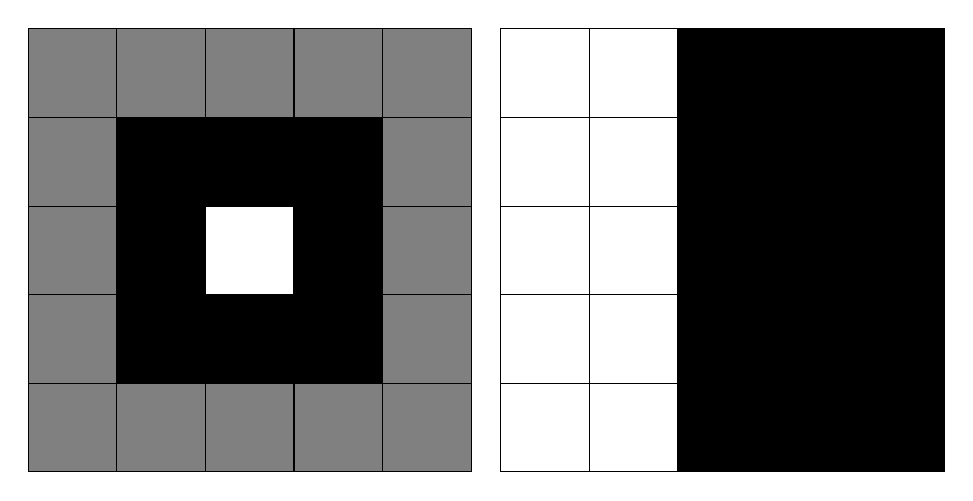
\begin{tikzpicture}
\node at (0,0)[rectangle,text width=0.9cm,text height=0.9cm,draw=black,fill=gray,align=center](00){};
\node at (0,1.125)[rectangle,text width=0.9cm,text height=0.9cm,draw=black,fill=gray,align=center](01){};
\node at (0,2.25)[rectangle,text width=0.9cm,text height=0.9cm,draw=black,fill=gray,align=center](02){};
\node at (0,3.375)[rectangle,text width=0.9cm,text height=0.9cm,draw=black,fill=gray,align=center](04.5){};
\node at(0,4.5)[rectangle,text width=0.9cm,text height=0.9cm,draw=black,fill=gray,align=center](04){};
\node at (1.125,0)[rectangle,text width=0.9cm,text height=0.9cm,draw=black,fill=gray,align=center](10){};
\node at (1.125,1.125)[rectangle,text width=0.9cm,text height=0.9cm,draw=black,fill=black,align=center](11){};
\node at (1.125,2.25)[rectangle,text width=0.9cm,text height=0.9cm,draw=black,fill=black,align=center](12){};
\node at (1.125,3.375)[rectangle,text width=0.9cm,text height=0.9cm,draw=black,fill=black,align=center](14.5){};
\node at(1.125,4.5)[rectangle,text width=0.9cm,text height=0.9cm,draw=black,fill=gray,align=center](14){};
\node at (2.25,0)[rectangle,text width=0.9cm,text height=0.9cm,draw=black,fill=gray,align=center](20){};
\node at (2.25,1.125)[rectangle,text width=0.9cm,text height=0.9cm,draw=black,fill=black,align=center](21){};
\node at (2.25,2.25)[rectangle,text width=0.9cm,text height=0.9cm,draw=black,fill=white,align=center](22){};
\node at (2.25,3.375)[rectangle,text width=0.9cm,text height=0.9cm,draw=black,fill=black,align=center](24.5){};
\node at(2.25,4.5)[rectangle,text width=0.9cm,text height=0.9cm,draw=black,fill=gray,align=center](24){};
\node at (3.375,0)[rectangle,text width=0.9cm,text height=0.9cm,draw=black,fill=gray,align=center](4.50){};
\node at (3.375,1.125)[rectangle,text width=0.9cm,text height=0.9cm,draw=black,fill=black,align=center](4.51){};
\node at (3.375,2.25)[rectangle,text width=0.9cm,text height=0.9cm,draw=black,fill=black,align=center](4.52){};
\node at (3.375,3.375)[rectangle,text width=0.9cm,text height=0.9cm,draw=black,fill=black,align=center](4.54.5){};
\node at(3.375,4.5)[rectangle,text width=0.9cm,text height=0.9cm,draw=black,fill=gray,align=center](4.54){};
\node at (4.5,0)[rectangle,text width=0.9cm,text height=0.9cm,draw=black,fill=gray,align=center](40){};
\node at (4.5,1.125)[rectangle,text width=0.9cm,text height=0.9cm,draw=black,fill=gray,align=center](41){};
\node at (4.5,2.25)[rectangle,text width=0.9cm,text height=0.9cm,draw=black,fill=gray,align=center](42){};
\node at (4.5,3.375)[rectangle,text width=0.9cm,text height=0.9cm,draw=black,fill=gray,align=center](44.5){};
\node at(4.5,4.5)[rectangle,text width=0.9cm,text height=0.9cm,draw=black,fill=gray,align=center](44){};
\node at (6,0)[rectangle,text width=0.9cm,text height=0.9cm,draw=black,fill=white,align=center](00){};
\node at (6,1.125)[rectangle,text width=0.9cm,text height=0.9cm,draw=black,fill=white,align=center](01){};
\node at (6,2.25)[rectangle,text width=0.9cm,text height=0.9cm,draw=black,fill=white,align=center](02){};
\node at (6,3.375)[rectangle,text width=0.9cm,text height=0.9cm,draw=black,fill=white,align=center](04.5){};
\node at(6,4.5)[rectangle,text width=0.9cm,text height=0.9cm,draw=black,fill=white,align=center](04){};
\node at (7.125,0)[rectangle,text width=0.9cm,text height=0.9cm,draw=black,fill=white,align=center](10){};
\node at (7.125,1.125)[rectangle,text width=0.9cm,text height=0.9cm,draw=black,fill=white,align=center](11){};
\node at (7.125,2.25)[rectangle,text width=0.9cm,text height=0.9cm,draw=black,fill=white,align=center](12){};
\node at (7.125,3.375)[rectangle,text width=0.9cm,text height=0.9cm,draw=black,fill=white,align=center](14.5){};
\node at (7.125,4.5)[rectangle,text width=0.9cm,text height=0.9cm,draw=black,fill=white,align=center](14){};
\node at (8.25,0)[rectangle,text width=0.9cm,text height=0.9cm,draw=black,fill=black,align=center](20){};
\node at (8.25,1.125)[rectangle,text width=0.9cm,text height=0.9cm,draw=black,fill=black,align=center](21){};
\node at (8.25,2.25)[rectangle,text width=0.9cm,text height=0.9cm,draw=black,fill=black,align=center](22){};
\node at (8.25,3.375)[rectangle,text width=0.9cm,text height=0.9cm,draw=black,fill=black,align=center](24.5){};
\node at (8.25,4.5)[rectangle,text width=0.9cm,text height=0.9cm,draw=black,fill=black,align=center](24){};
\node at (9.375,0)[rectangle,text width=0.9cm,text height=0.9cm,draw=black,fill=black,align=center](4.50){};
\node at (9.375,1.125)[rectangle,text width=0.9cm,text height=0.9cm,draw=black,fill=black,align=center](4.51){};
\node at (9.375,2.25)[rectangle,text width=0.9cm,text height=0.9cm,draw=black,fill=black,align=center](4.52){};
\node at (9.375,3.375)[rectangle,text width=0.9cm,text height=0.9cm,draw=black,fill=black,align=center](4.54.5){};
\node at (9.375,4.5)[rectangle,text width=0.9cm,text height=0.9cm,draw=black,fill=black,align=center](4.54){};
\node at (10.5,0)[rectangle,text width=0.9cm,text height=0.9cm,draw=black,fill=black,align=center](40){};
\node at (10.5,1.125)[rectangle,text width=0.9cm,text height=0.9cm,draw=black,fill=black,align=center](41){};
\node at (10.5,2.25)[rectangle,text width=0.9cm,text height=0.9cm,draw=black,fill=black,align=center](42){};
\node at (10.5,3.375)[rectangle,text width=0.9cm,text height=0.9cm,draw=black,fill=black,align=center](44.5){};
\node at (10.5,4.5)[rectangle,text width=0.9cm,text height=0.9cm,draw=black,fill=black,align=center](44){};
\end{tikzpicture}
\end{center}
\caption{Receptive field and visual stimulus.\label{fig:stim}}
\end{figure}


\begin{thebibliography}{10}

\bibitem{HubelWiesel1962a} Hubel DH, Wiesel TN. (1962) Receptive
  fields, binocular interaction and functional architecture in the
  cat's visual cortex.  \newblock The Journal of Physiology 160: 106.

\end{thebibliography}

\end{document}

